\documentclass{article}
\usepackage{bm}
\usepackage{amsmath}
\usepackage{graphicx}
\usepackage[left=25mm,right=25mm,top=25mm,bottom=25mm,paper=a4paper]{geometry}

\graphicspath{ {C:\Users\qwert\OneDrive\Documents\GitHub\ThreeBodyProblemVis\Images\averages1to100.png}}
\author{Caedan Miller, Kiki Murphy, Will St. John}
\title{MATH 312 Final Project Paper}

\begin{document}
\maketitle
\tableofcontents
\newpage
\section{Project Overview}
\subsection{Introduction}
The three body problem describes the problem of finding the positions of three objects with individual masses, initial positions, and initial velocities using Newtonian laws of motion and gravity. Unlike two body problems, closed-form solutions do not exist for the three body problem. In our case, this means that the positions of the three bodies must be approximated using numerical methods. In this paper, we will explore numerical solutions to the three body problem in two dimensions using Heun's Method. We will also explore the three body problem in two dimensions with the addition of masses and the gravitational constant $G$.


\subsection{Equations}
Newton's law of universal gravitation states that the gravitational force between two objects is proportional to the product of their masses and inversely proportional to the square of the distance between them. For object one in our system, this can be expressed mathematically as follows:
\begin{equation}
    \bm{F_{g,1}} = -G\frac{m_1 m_2}{|\bm{r_{12}}|^2}\bm{\hat{r_{21}}} -G\frac{m_1 m_3}{|\bm{r_{13}}|^2}\bm{\hat{r_{31}}}
\end{equation}
where $\bm{F_g}$ is the gravitational force between two objects, $G$ is the gravitational constant, $m_1$ and $m_2$ are the masses of the two objects, and $\bm{r}$ is the distance between the two objects.

The positional vector from one object to the next can be described as the difference in position vectors for the two objects. In other words:
\begin{equation}
    \bm{r_{12}} = \bm{r_1} - \bm{r_2}
\end{equation}

Additionally, the unit vector $\bm{\hat{r}}$ can be expressed as the positional vector divided by its magnitude.
\begin{equation}
    \bm{\hat{r}} = \frac{\bm{r}}{|\bm{r}|}
\end{equation}

Using equations (2) and (3), equation (1) can be rewritten as follows:

\begin{equation}
    \bm{F_{g,1}} = -Gm_1 m_2\frac{\bm{r_1} - \bm{r_2}}{|\bm{r_1} - \bm{r_2}|^3}-Gm_1 m_3\frac{\bm{r_1} - \bm{r_3}}{|\bm{r_1} - \bm{r_3}|^3}
\end{equation}


Newton's second law of motion states that the acceleration of an object is proportional to the net force acting on it and inversely proportional to its mass. This can be expressed mathematically as follows:
\begin{equation}
    \bm{F_{net}} = m\bm{a}
\end{equation}
where $F_{net}$ is the net force acting on an object, $m$ is the mass of the object, and $a$ is the acceleration of the object.

Setting equation (5) with $m=m_1$ equal to equation (4) and solving for acceleration yields the following relationship for the acceleration of object one:

\begin{align}
    \bm{F_{net,1}} &= \bm{F_{g,1}} \nonumber \\
    m_1\bm{a_1} &= -Gm_1 m_2\frac{\bm{r_1} - \bm{r_2}}{|\bm{r_1} - \bm{r_2}|^3}-Gm_1 m_3\frac{\bm{r_1} - \bm{r_3}}{|\bm{r_1} - \bm{r_3}|^3}\nonumber \\
    \bm{a_1} &= -Gm_2\frac{\bm{r_1} - \bm{r_2}}{|\bm{r_1} - \bm{r_2}|^3}-Gm_3\frac{\bm{r_1} - \bm{r_3}}{|\bm{r_1} - \bm{r_3}|^3}
\end{align}

Similar equations can be found for the other two objects in the system.  The result are three second-order differential equations can model the three body problem as described by Newtonian mechanics. These equations are as follows:

\begin{align}
    \ddot{\bm{r_1}} &= -Gm_2\frac{\bm{r_1}-\bm{r_2}}{|\bm{r_1}-\bm{r_2}|^3}-Gm_3\frac{\bm{r_1}-\bm{r_3}}{|\bm{r_1}-\bm{r_3}|^3}\\
    \ddot{\bm{r_2}} &= -Gm_1\frac{\bm{r_2}-\bm{r_1}}{|\bm{r_2}-\bm{r_1}|^3}-Gm_3\frac{\bm{r_2}-\bm{r_3}}{|\bm{r_2}-\bm{r_3}|^3}\\
    \ddot{\bm{r_1}} &= -Gm_1\frac{\bm{r_3}-\bm{r_1}}{|\bm{r_3}-\bm{r_1}|^3}-Gm_2\frac{\bm{r_3}-\bm{r_2}}{|\bm{r_3}-\bm{r_2}|^3}
\end{align}

where $r_1$, $r_2$, and $r_3$ are the vector positions of the three bodies, $m_1$, $m_2$, and $m_3$ are the masses of the three bodies, and $G$ is the gravitational constant.

\subsection{Simplification}
To simplify the problem, we assume the following conditions:
\begin{itemize}
    \item The three bodies only move in two dimensions.
    \item The three bodies are of equal mass $m_1 = m_2 = m_3 = 1$.
    \item The gravitational constant $G = 1$.
\end{itemize}

Equations (1), (2), and (3) can be rewritten as follows:
\begin{align}
    \ddot{r_1} &= -\frac{r_1-r_2}{|r_1-r_2|^3}-\frac{r_1-r_3}{|r_1-r_3|^3}\\
    \ddot{r_2} &= -\frac{r_2-r_1}{|r_2-r_1|^3}-\frac{r_2-r_3}{|r_2-r_3|^3}\\
    \ddot{r_3} &= -\frac{r_3-r_1}{|r_3-r_1|^3}-\frac{r_3-r_2}{|r_3-r_2|^3}
\end{align}

\subsection{Goals}
Our intended goal was to model the three body problem in the 2D plane for a range of initial conditions using Heun's Method. Once every approximation is complete, we would create a “moment map” of the result by averaging the amount of times a planet appears at a particular pixel and giving that pixel a corresponding RGB value. For example, a pixel where planet 1 (red) passes through numerous times would appear very dark red in the moment map, while a pixel where planet 1 (red) and 3 (blue) pass through a lot would appear purple.The steps towards this goal fall into two categories: those that we are certain we can achieve and those that are more ambitious.


The minimum viable product (MVP) of our project entails (1) rewritten equations for the three-body problem in two dimensions, (2) code in python to compute Heun's equations for all 12 of the three-body equations, and (3) plots of three-body motion featuring all three bodies and the center of mass in Python. 

\section{Process}
Our more ambitious goals entail the creation of the RGB map synthesizing the motion of the three bodies over a variety of initial conditions in order to achieve a better understanding of how the bodies tend to move. 
\subsection{Code}
\subsubsection{Necessary Packages}
\begin{verbatim}
import pandas as pd
import matplotlib.pyplot as plt
import numpy as np
import random
\end{verbatim}

\subsubsection{Heun's Method}
\begin{verbatim}
def heun(p0: np.array, N: int, t: float) -> np.array:
    """Calculatue heuns method for the three body problem for N steps with step size t.

    Args:
        p0 (np.array): 12 dimensional vector of initial conditions corresponding to the following:
            p0[0] = x1, p0[1] = x2, p0[2] = x3, p0[3] = y1, p0[4] = y2, p0[5] = y3, 
            p0[6] = vx1, p0[7] = vx2, p0[8] = vx3, p0[9] = vy1, p0[10] = vy2, p0[11] = vy3
        N (int): number of steps
        t (float): step size

    Returns:
        np.array: np.array positions and velocities for each x and y of each planet
    """
    data = [p0[0], p0[1], p0[2], p0[3], p0[4], p0[5], 
            p0[6], p0[7], p0[8], p0[9], p0[10], p0[11], 
            derivative(p0)[6], derivative(p0)[7], derivative(p0)[8], 
            derivative(p0)[9], derivative(p0)[10], derivative(p0)[11]]
    df = pd.DataFrame(data=[data], columns=['P1: X Position', 'P2: X Position', 
                                'P3: X Position', 'P1: Y Position', 'P2: Y Position', 
                                'P3: Y Position', 'P1: X Velocity', 'P2: X Velocity', 
                                'P3: X Velocity', 'P1: Y Velocity', 'P2: Y Velocity', 
                                'P3: Y Velocity', 'P1: X Acceleration', 'P2: X Acceleration', 
                                'P3: X Acceleration', 'P1: Y Acceleration', 'P2: Y Acceleration', 
                                'P3: Y Acceleration'])

    for i in range(0, N):
        ptemp = p0 + t * derivative(p0)
        dp0 = derivative(p0)
        dptemp = derivative(ptemp)
        p0 = p0 + t/2 * (dp0 + dptemp)
        data = [p0[0], p0[1], p0[2], p0[3], p0[4], p0[5], p0[6], p0[7], p0[8], p0[9], p0[10], p0[11], 
            derivative(p0)[6], derivative(p0)[7], derivative(p0)[8], derivative(p0)[9], derivative(p0)[10], 
            derivative(p0)[11]]
        df2 = pd.DataFrame(data=[data], columns=['P1: X Position', 'P2: X Position', 
                                'P3: X Position', 'P1: Y Position', 'P2: Y Position', 
                                'P3: Y Position', 'P1: X Velocity', 'P2: X Velocity', 
                                'P3: X Velocity', 'P1: Y Velocity', 'P2: Y Velocity', 
                                'P3: Y Velocity', 'P1: X Acceleration', 'P2: X Acceleration', 
                                'P3: X Acceleration', 'P1: Y Acceleration', 'P2: Y Acceleration', 
                                'P3: Y Acceleration'])
        df2['P1: X Position'] = p0[0]
        df2['P2: X Position'] = p0[1]
        df2['P3: X Position'] = p0[2]
        df2['P1: Y Position'] = p0[3]
        df2['P2: Y Position'] = p0[4]
        df2['P3: Y Position'] = p0[5]
        df2['P1: X Velocity'] = p0[6]
        df2['P2: X Velocity'] = p0[7]
        df2['P3: X Velocity'] = p0[8]
        df2['P1: Y Velocity'] = p0[9]
        df2['P2: Y Velocity'] = p0[10]
        df2['P3: Y Velocity'] = p0[11]
        df = pd.concat([df, df2], ignore_index=True)
    
    df.insert(0, 'Time', [i * t for i in range(0, N + 1)])
    return df
\end{verbatim}

\subsubsection{Derivative}
\begin{verbatim}
def derivative(p0: np.array) -> np.array:
    """Calculates the derivative of the 12 dimensional vector p0.

    Args:
        p0 (np.array): 12 dimensional vecotr of initial conditions corresponding to the following:
            p0[0] = x1, p0[1] = x2, p0[2] = x3, p0[3] = y1, p0[4] = y2, p0[5] = y3, 
            p0[6] = vx1, p0[7] = vx2, p0[8] = vx3, p0[9] = vy1, p0[10] = vy2, p0[11] = vy3 

    Returns:
        np.array: 12 dimensional vector of the derivative of p0
    """
    p1 = 0 * p0
    p1[0] = p0[6]
    p1[1] = p0[7]
    p1[2] = p0[8]
    p1[3] = p0[9]
    p1[4] = p0[10]
    p1[5] = p0[11]
    p1[6] = - ((p0[0] - p0[1])/((p0[0]-p0[1])**2+(p0[3]-p0[4])**2)**(3/2)) - ((p0[0] - p0[2])/((p0[0]-p0[2])**2+(p0[3]-p0[5])**2)**(3/2))
    p1[7] = - ((p0[1] - p0[0])/((p0[1]-p0[0])**2+(p0[4]-p0[3])**2)**(3/2)) - ((p0[1] - p0[2])/((p0[1]-p0[2])**2+(p0[4]-p0[5])**2)**(3/2))
    p1[8] = - ((p0[2] - p0[0])/((p0[2]-p0[0])**2+(p0[5]-p0[3])**2)**(3/2)) - ((p0[2] - p0[1])/((p0[2]-p0[1])**2+(p0[5]-p0[4])**2)**(3/2))
    p1[9] = - ((p0[3] - p0[4])/((p0[0]-p0[1])**2+(p0[3]-p0[4])**2)**(3/2)) - ((p0[3] - p0[5])/((p0[0]-p0[2])**2+(p0[3]-p0[5])**2)**(3/2))
    p1[10] = - ((p0[4] - p0[3])/((p0[1]-p0[0])**2+(p0[4]-p0[3])**2)**(3/2)) - ((p0[4] - p0[5])/((p0[1]-p0[2])**2+(p0[4]-p0[5])**2)**(3/2))
    p1[11] = - ((p0[5] - p0[3])/((p0[2]-p0[0])**2+(p0[5]-p0[3])**2)**(3/2)) - ((p0[5] - p0[4])/((p0[2]-p0[1])**2+(p0[5]-p0[4])**2)**(3/2))
    return p1
\end{verbatim}

\subsubsection{Perterbations}
\begin{verbatim}
def perterbations(N: int) -> list:
    """Randomly generates N positions within the first two quadrants of a circle 
        with radius less than or equal to 0.01.

    Args:
        N (int): number of positions to generate

    Returns:
        list: tuples of x and y positions
    """
    positions = []
    while len(positions) < N:
        x = random.randrange(-1000, 1000, 1) / 10000
        y = random.randrange(0, 1000, 1) / 10000
        if x**2 + y**2 <= 0.01:
            positions.append((x, y))
    return positions
\end{verbatim}

\subsubsection{Making Plots}
\begin{verbatim}
    def make_vis(pos: int, pert: int, title: str) -> None:
    """Creates a visualization of the three body problem with pert perturbations. Indended 
    to be used with subplots.

    Args:
        pos (int): subplot position for the visualization
        pert (int): number of perterbations to include in the plot
        title (str): title of the plot
    """
    mid_pos = perterbations(pert)

    p = np.array([-1, 1, 0, 0, 0, 0, 0, 0, 0, -1, 1, 0])
    d = heun(p, 5000, 0.001)
    plt.subplot(pos)

    plt.title(title)
    plt.plot(d['P1: X Position'][0], d['P1: Y Position'][0], c='red', marker='x', label='Earth')
    plt.plot(d['P2: X Position'][0], d['P2: Y Position'][0], c='green', marker='x',label='Mars')
    plt.plot(d['P3: X Position'][0], d['P3: Y Position'][0], c='blue', marker='x', label='Venus')
    plt.plot(d['P1: X Position'], d['P1: Y Position'], c='red', alpha=0.3, label='Earth')
    plt.plot(d['P2: X Position'], d['P2: Y Position'], c='green', alpha=0.3, label='Mars')
    plt.plot(d['P3: X Position'], d['P3: Y Position'], c='blue', alpha=0.3, label='Venus')

    for x, y in mid_pos:
        p = np.array([-1, 1, x, 0, 0, y, 0, 0, 0, -1, 1, 0])
        d = heun(p, 5000, 0.001)        
        plt.plot(d['P1: X Position'], d['P1: Y Position'], c='red', alpha=0.5)
        plt.plot(d['P2: X Position'], d['P2: Y Position'], c='green', alpha=0.5)
        plt.plot(d['P3: X Position'], d['P3: Y Position'], c='blue', alpha=0.5)
    return
\end{verbatim}

\subsubsection{Making Average Plots}
\begin{verbatim}
def generate_avg(pert: int, pos: int, duration: int, stepsize: float) -> None:
    """Creates an average of pert perterbations using Heun's method for a particular duration and stepsize.

    Args:
        pert (int): number of perterbations to plot
        duration (int): how many steps to take
        stepsize (float): step size for heun's method
    """
    x1 = []
    x2 = []
    x3 = []
    y1 = []
    y2 = []
    y3 = []
    mid_pos = perterbations(pert)
    plt.subplot(pos)

    for x, y in mid_pos:
            p = np.array([-1, 1, x, 0, 0, y, 0, 0, 0, -1, 1, 0])
            d = heun(p, duration, stepsize)
            x1.append(d['P1: X Position'])
            x2.append(d['P2: X Position'])
            x3.append(d['P3: X Position'])
            y1.append(d['P1: Y Position'])
            y2.append(d['P2: Y Position'])
            y3.append(d['P3: Y Position'])
            plt.plot(d['P1: X Position'], d['P1: Y Position'], c='red', alpha=0.1)
            plt.plot(d['P2: X Position'], d['P2: Y Position'], c='green', alpha=0.1)
            plt.plot(d['P3: X Position'], d['P3: Y Position'], c='blue', alpha=0.1)

    x1avg = np.mean(x1, axis=0)
    x2avg = np.mean(x2, axis=0)
    x3avg = np.mean(x3, axis=0)
    y1avg = np.mean(y1, axis=0)
    y2avg = np.mean(y2, axis=0)
    y3avg = np.mean(y3, axis=0)

    plt.title(f"Average of {pert} Perturbations")
    plt.plot(x1avg, y1avg, c='red', alpha=1)
    plt.plot(x2avg, y2avg, c='green', alpha=1)
    plt.plot(x3avg, y3avg, c='blue', alpha=1)
    return
\end{verbatim}

\subsection{Adding Masses \& G}

\subsection{Exploring Collinear Initial Conditions}
Talk about stable colinear solutions found online

\section{Results and Discussion}
\begin{figure}[h!]
    \centering
    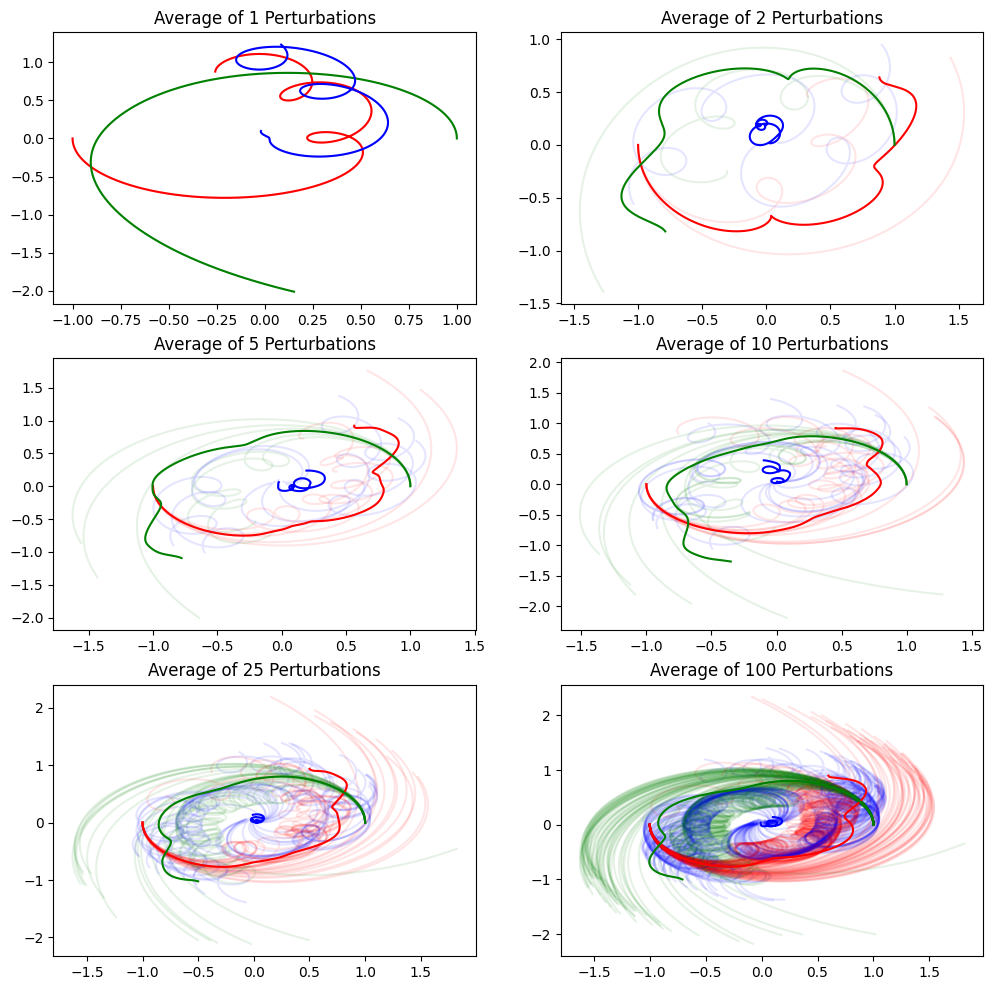
\includegraphics[width=0.8\textwidth]{Images/averages1to100.png}
    \caption{a nice plot}
    \label{fig:mesh1}
\end{figure}

\begin{figure}[h!]
    \centering
    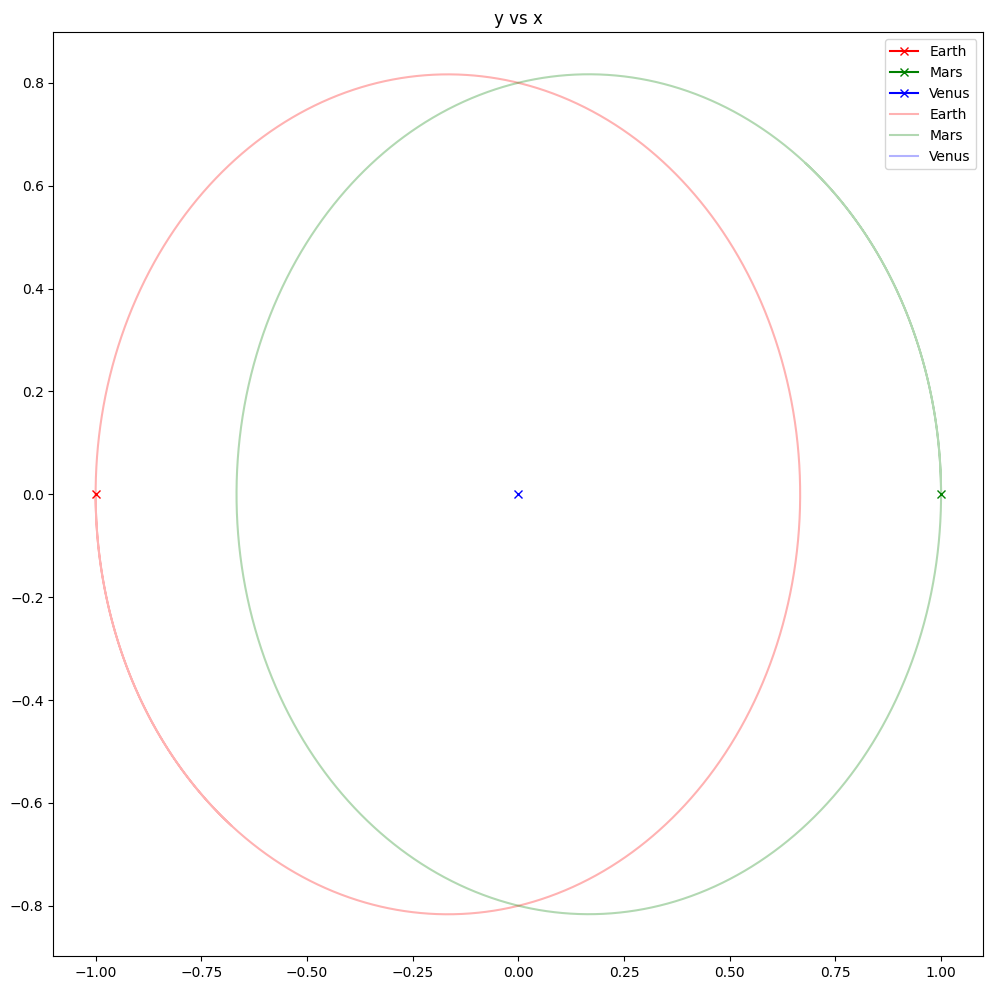
\includegraphics[width=0.8\textwidth]{Images/noPerterbations.png}
    \caption{a nice plot}
    \label{fig:mesh2}
\end{figure}

\begin{figure}[h!]
    \centering
    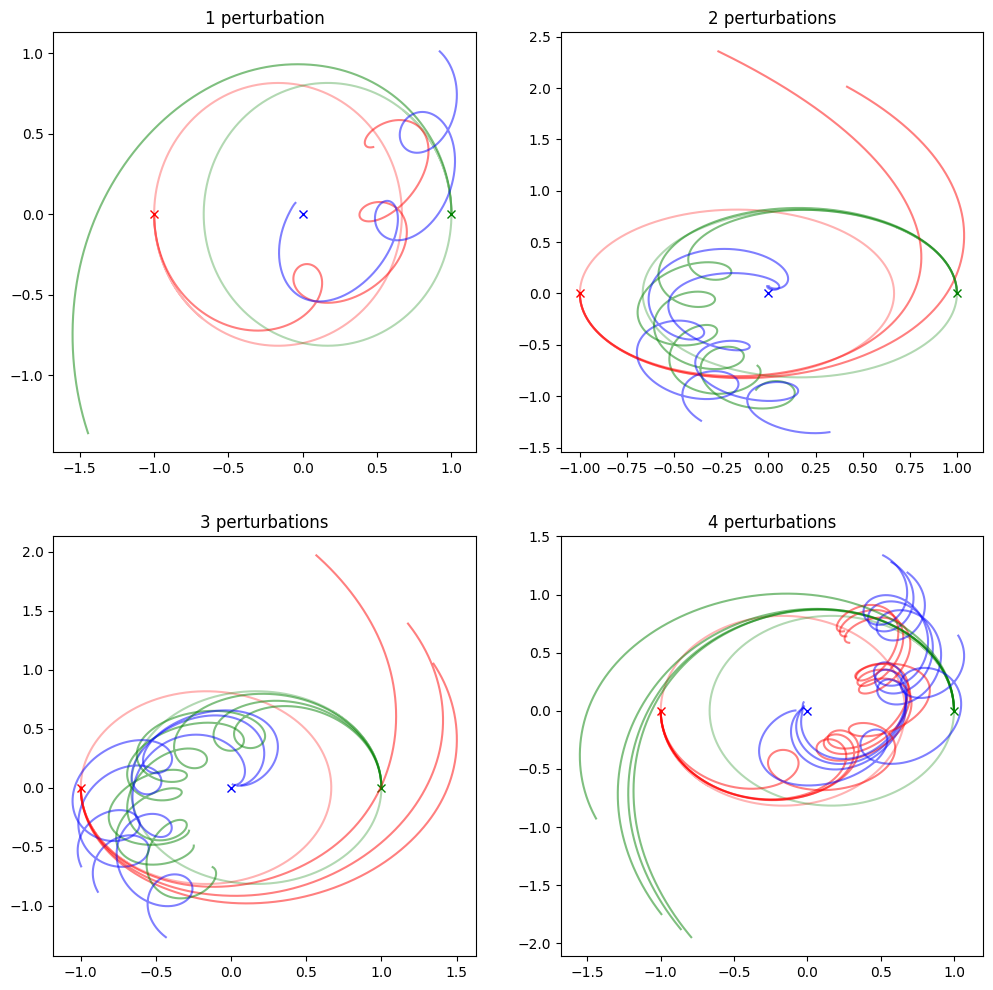
\includegraphics[width=0.8\textwidth]{Images/perterbations1to4.png}
    \caption{a nice plot}
    \label{fig:mesh3}
\end{figure}

\section{Conclusion}

\end{document}